\section{Application 1: Whitened Variational Gaussian Processes}
\label{sec:variational_results}

As a first application of the CIQ method, we will demonstrate that the scalable whitening procedure $\bK^{-1/2} \bb$ can accelerate and increase the fidelity of variational Gaussian process approximations.
The whitening operation is commonly used with variational approximations to accelerate the learning of variational parameters \cite{matthews2017gpflow}.


\paragraph{Whitened Stochastic Variational Gaussian Processes.}
Rather than directly learning $\bm$ and $\bS$, it is more common to learn the \emph{whitened parameters} \cite{kuss2005assessing,matthews2017scalable}:
\[ \bm' = \bK^{-\frac 1 2} \bm, \quad \bS' = \bK^{-\frac 1 2} \bS \bK^{-\frac 1 2} \]
Under this coordinate system, the KL divergence term is given by
%
\begin{equation}
	\kl{ q(\bu') }{ p(\bu') } = \frac{1}{2} \Bigl( \bm^{\prime \top} \bm' + \tr{ \bS' } - \log \vert \bS' \vert - M \Bigr),
	\label{eqn:kldiv_whitened}
\end{equation}
%
which importantly does not depend on $k(\cdot,\cdot)$ or $\bZ$ and therefore is relatively simple to optimize.
The whitened predictive mean and variance become
%
\begin{align}
  \ameantest{\bx} &= \bk_{\bZ\bx}^\top \bK^{-\frac 1 2} \bm'
  \label{eqn:approx_pred_mean} \\
  \avartest{\bx} &= k(\bx, \bx) -
    \bk_{\bZ\bx}^\top \bK^{-\frac 1 2} \left( \bI - \bS' \right) \bK^{-\frac 1 2} \bk_{\bZ\bx}
  \label{eqn:approx_pred_covar}
\end{align}

During optimization, we must compute the predictive distribution of every data point $\bx_i, y_i$.
This requires computing $\bK^{- \frac 1 2} \bk_{\bX \bx_i}$ and its derivative for every $\bx_i$ at every optimization iteration.\footnote{
  Since SVGP is compatible with minibatch optimization, we often only compute $\bK^{- \frac 1 2} \bk_{\bZ \bx_i}$ for a fraction of the training data.
}
This can computed using the Cholesky decomposition (up to an orthogonal rotation) or CIQ.

\gp{Stopped here.}

\begin{figure}[t!]
  \centering
  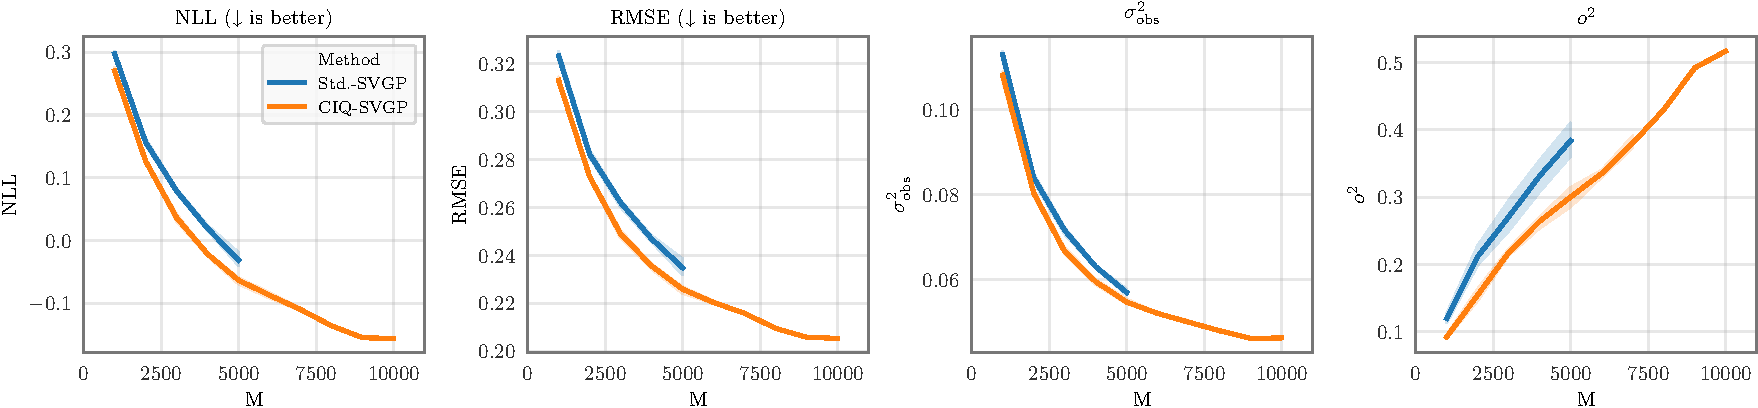
\includegraphics[width=\linewidth]{figures/3droad.pdf}
  \caption{
    SVGP models trained on the 3D-Road dataset ($D=2$, $N\geq300,\!000$), varying $M$ (the number of inducing points).
    \gp{FINISH}
  }
  \label{fig:3droad}
\end{figure}

\begin{figure}[t!]
  \centering
  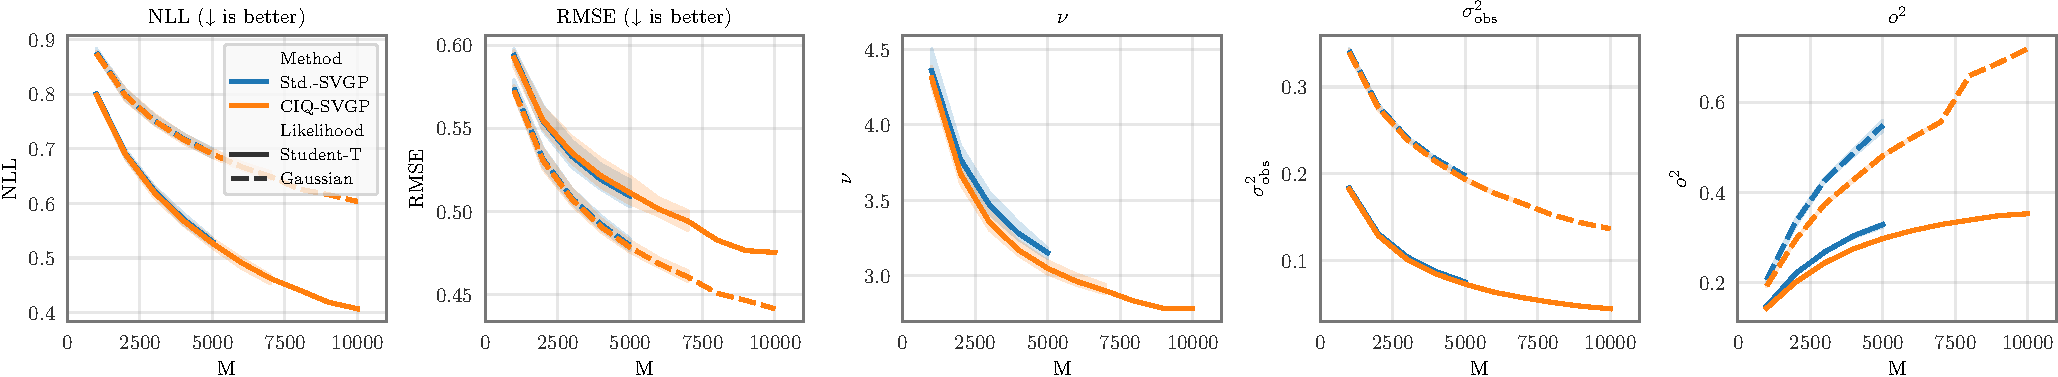
\includegraphics[width=\linewidth]{figures/precip.pdf}
  \caption{
    SVGP models trained on the Precipitation dataset ($D=3$, $N\geq300,\!000$), varying $M$ (the number of inducing points).
    \gp{FINISH}
  }
  \label{fig:precip}
\end{figure}

\begin{figure}[t!]
  \centering
  \caption{
    SVGP models trained on the Robotics dataset ($D=?$, $N\geq?$), varying $M$ (the number of inducing points).
    \gp{FINISH}
  }
  \label{fig:robotics}
\end{figure}
